\tinypar{Summary} \textbf{Angelo Porrello} è membro da sette anni del gruppo di ricerca \href{https://aimagelab.ing.unimore.it/imagelab/}{\textbf{AImageLab}} presso il Dipartimento di Ingegneria “Enzo Ferrari” dell’Università di Modena e Reggio Emilia. Attualmente ricopre il ruolo di Ricercatore a Tempo Determinato di Tipo A (RTD-A). Svolge un'attività di ricerca continuativa e riconosciuta a livello internazionale nei settori dell’\textit{Artificial Intelligence} e della \textit{Computer Vision}. È autore di oltre quaranta pubblicazioni scientifiche sottoposte a revisione paritaria, apparse su riviste e conferenze internazionali di primo piano (tra cui CVPR, ECCV, ICCV, NeurIPS, ICLR). Le sue principali linee di ricerca riguardano lo sviluppo di tecniche e metodi avanzati per l’\textbf{addestramento di reti neurali}, con particolare riferimento a \textit{continual learning}, \textit{modular deep learning} e \textit{federated learning}. Si occupa inoltre di sistemi di AI e Computer Vision applicati all’\textit{anomaly detection} e alla \textit{video analytics}.

\vspace{0.5em}
\tinypar{Abilitazione Scientifica Nazionale} Ha conseguito l’Abilitazione Scientifica Nazionale alle funzioni di Professore di Seconda Fascia nei settori concorsuali \textbf{01/B1} (Informatica) e \textbf{09/H1} (Sistemi di Elaborazione delle Informazioni).

%Nel biennio 2022-2023 è stato advisor scientifico di \href{https://cristail.com/it/}{Cristail}, startup che si occupa di sviluppare strumenti di asset management intelligenti attraverso tecniche avanzate di AI. 
%
\section{Profilo Scholar}
%
Metriche aggiornate al 12/01/2026.
\vspace{-0.8em}
\begin{center}
\begin{tabular}{cc}
     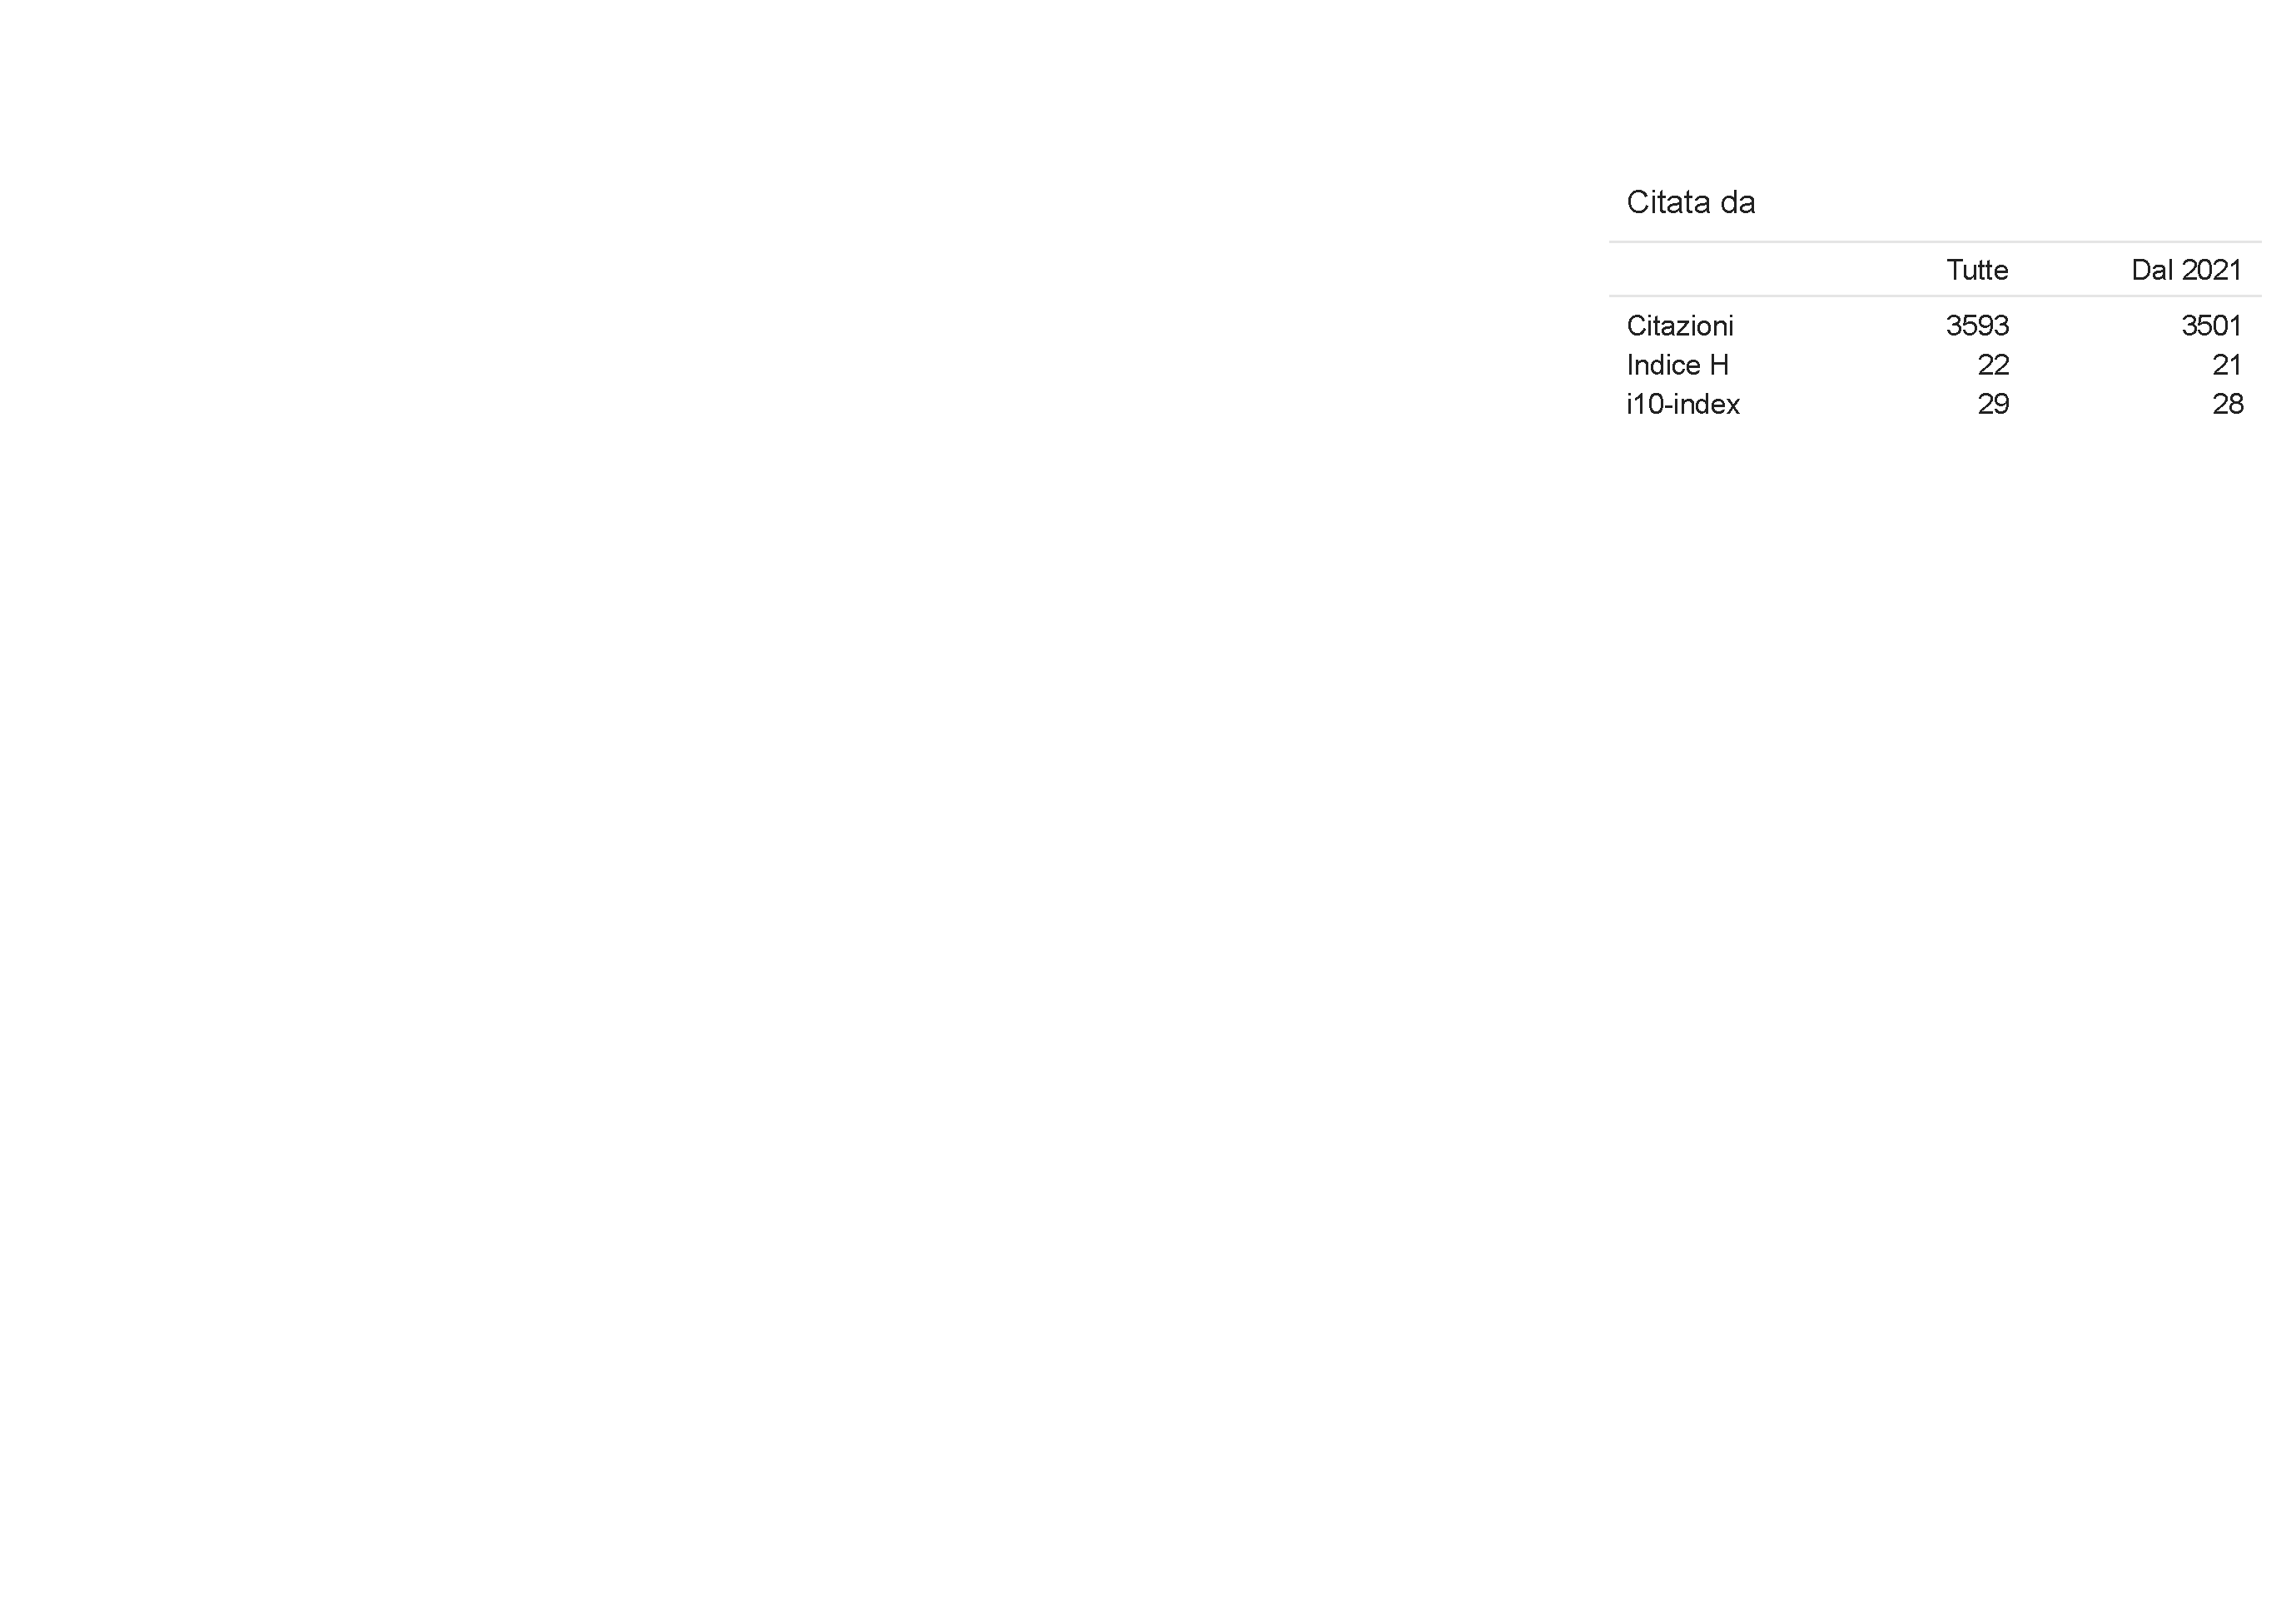
\includegraphics[width=0.55\textwidth]{images/scholar-numbers.pdf} & 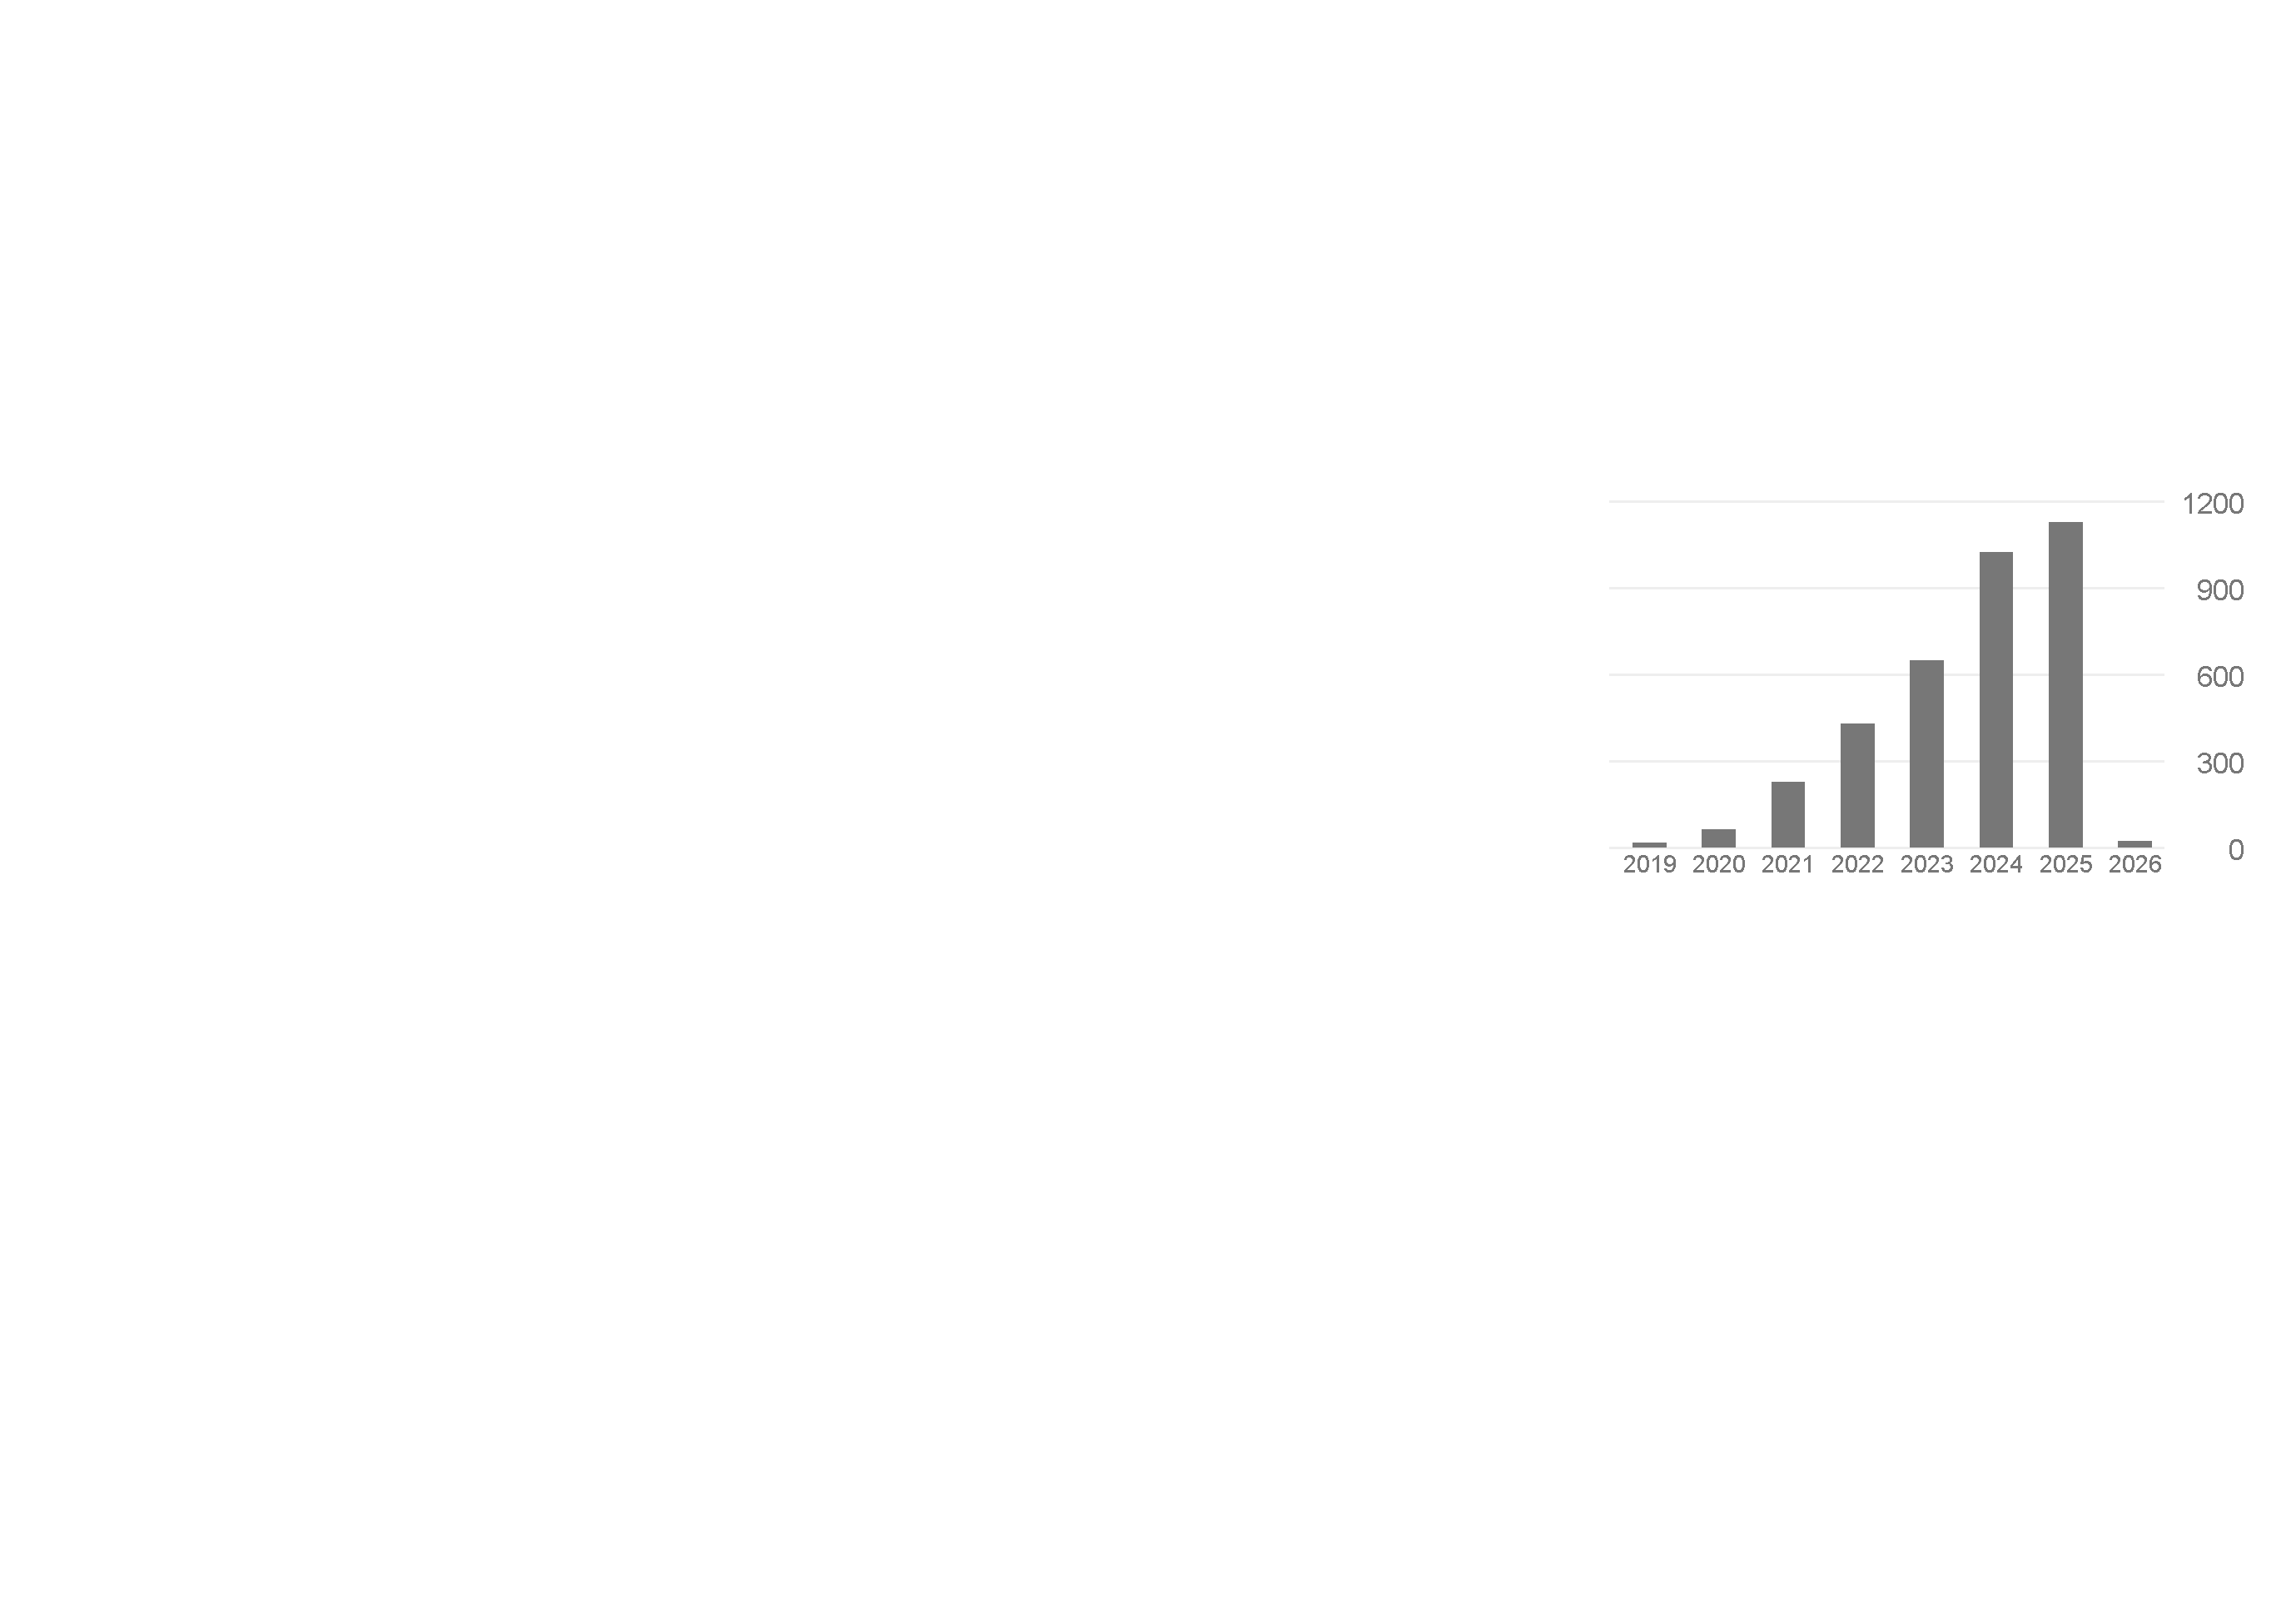
\includegraphics[width=0.4\textwidth]{images/scholar-plot.pdf}
\end{tabular}    
\end{center}